\documentclass{article}
\usepackage{ml1_homework_template}
\usepackage{amsmath}
\usepackage{amssymb}
% please submit the corresponding pdf by email to
% homework@class,brml.org, and write "homework sheet xx" in the 
% title.  No more, no less!  (Instead of xx, however,
% put the decimal number of the homework sheet.)

% Please update the following line, only change XX to the homework
% sheet number
\title{homework sheet 09}


\author{
\name{Andre Seitz}\\
\imat{03622870}\\
\email{andre.seitz@mytum.de}
\And
\name{Linda Leidig} \\
\imat{03608416}\\
\email{linda.leidig@tum.de}
}

% The \author macro works with any number of authors. There are two commands
% used to separate the names and addresses of multiple authors: \And and \AND.
%
% Using \And between authors leaves it to \LaTeX{} to determine where to break
% the lines. Using \AND forces a linebreak at that point. So, if \LaTeX{}
% puts 3 of 4 authors names on the first line, and the last on the second
% line, try using \AND instead of \And before the third author name.

\renewcommand{\Vec}[1]{\ensuremath{\mathbf{#1}}}
\newcommand{\Mtx}[1]{\ensuremath{\mathbf{#1}}}
\newcommand{\R}{\ensuremath{\mathbb{R}}}

\usepackage{graphicx}

\begin{document}
\maketitle

\section{Assignment: Optimization and Convexity}
\paragraph*{Problem 1}
$\;$ 

A function $f$ is strictly convex if the value of $f$ at any point between the two points $\Vec{x},\Vec{y} \in \mathcal{X}$ except themselves is smaller than the value of the linear function $g$ that intersects the two points $\Vec{x}$ and $\Vec{y}$ at the considered point. In contrast, convex functions are also allowed to lie directly on this linear function $g$. Therefore, a linear function is convex but not strictly convex and a strictly convex function is not allowed to have any linear parts.

\paragraph*{Problem 2}
$\;$ 

If a function $f(\Vec{x})$ is convex, at most infinite many $\Vec{x}^*$ can satisfy the equation $f(\Vec{x}^*) = min_xf(\Vec{x})$. In particular, this holds for constant functions that are convex functions per definition. Their value is the same for all possible $\Vec{x}^*$ which are infinite many. As the function has only one value this is the minimum value.

\paragraph*{Problem 3}
$\;$ 

If a function $f(\Vec{x})$ is strictly convex, there is exactly one $\Vec{x}^*$ that can satisfy the equation $f(\Vec{x}^*) = min_xf(\Vec{x})$. The only case that there are more than one $\Vec{x}^*$ fulfilling this condition is if the function consists of parts that are constant. But, this is not possible for strictly convex functions as they are not allowed to have linear parts as described in Problem 1. Since constant functions are also linear, there is only one $\Vec{x}^*$ that fulfils the condition $f(\Vec{x}^*) = min_xf(\Vec{x})$.

\paragraph*{Problem 4}
$\;$ 

strictly convex function: $f(x) = \frac{5}{7}x^2-10$\\
convex function: $g(x) = 4x$

See Figure \ref{convex}.

\begin{figure}[ht]
\centering
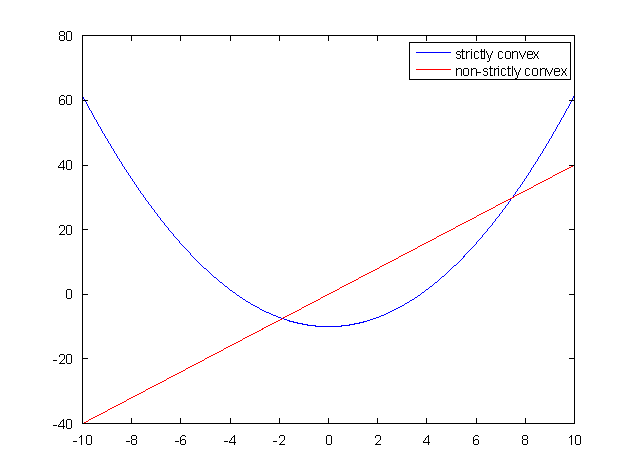
\includegraphics{convex.pdf}
\caption{A strictly convex and a non-strictly convex function.}
\label{convex}
\end{figure}


\section{Assignment: The Gaussian kernel for classification}
\paragraph*{Problem 5}
$\;$

No, it is not possible to apply this infinite dimensional feature map directly since it is not possible to express infinite many basis functions. Therefore, kernels or the dual representation is the solution as its complexity depends on the number of data samples rather than the number of basis functions which is in this case infinite.

\paragraph*{Problem 6}
$\;$ 

\begin{eqnarray}
&&K(x,y)\\
&=& \sum_{i=1}^{\infty} \Phi_{\infty,i}(x) \Phi_{\infty,i}(y)\\
&=& e^{\frac{-x^2}{2\sigma^2}}e^{\frac{-y^2}{2\sigma^2}} + e^{\frac{-x^2}{2\sigma^2}}\frac{x}{\sigma}e^{\frac{-y^2}{2\sigma^2}}\frac{y}{\sigma} + \frac{e^{\frac{-x^2}{2\sigma^2}}\left(\frac{x}{\sigma}\right)^2}{\sqrt{2}}\frac{e^{\frac{-y^2}{2\sigma^2}}\left(\frac{y}{\sigma}\right)^2}{\sqrt{2}}+...+ \frac{e^{\frac{-x^2}{2\sigma^2}}\left(\frac{x}{\sigma}\right)^i}{\sqrt{i!}}\frac{e^{\frac{-y^2}{2\sigma^2}}\left(\frac{y}{\sigma}\right)^i}{\sqrt{i!}}+...\\
&=& \frac{e^{\frac{-x^2-y^2}{2\sigma^2}}\left( \frac{xy}{\sigma^2} \right)^0}{0!} + \frac{e^{\frac{-x^2-y^2}{2\sigma^2}}\left( \frac{xy}{\sigma^2} \right)^1}{1!} + \frac{e^{\frac{-x^2-y^2}{2\sigma^2}}\left( \frac{xy}{\sigma^2} \right)^2}{2!} + ... + \frac{e^{\frac{-x^2-y^2}{2\sigma^2}}\left( \frac{xy}{\sigma^2} \right)^i}{i!} + ...\\
&=& \sum_{n = 0}^{\infty} \frac{e^{\frac{-x^2-y^2}{2\sigma^2}}\left( \frac{xy}{\sigma^2} \right)^n}{n!}\\
&=& e^{\frac{-x^2-y^2}{2\sigma^2}} \sum_{n = 0}^{\infty} \frac{\left( \frac{xy}{\sigma^2} \right)^n}{n!}\\ 
&=& e^{\frac{-x^2-y^2}{2\sigma^2}} e^{\frac{xy}{\sigma^2}}\\
&=& e^{\frac{-x^2-y^2+2xy}{2\sigma^2}}
\end{eqnarray}

Yes, with such high-dimensional feature space we should be concerned about overfitting.

\paragraph*{Problem 7}
$\;$ 

\section{Assignment: The SVM optimisation problem}
\paragraph*{Problem 8}
$\;$ 

\end{document}
